\section{Einleitung}
In dem Versuch wird der Reinst-Germanium-Detektor näher betrachtet. Dazu werden wichtige Kenngrößen, wie das energetische Auflösungsvermögen und die spektrale Empfindlichkeit, des Detektors bestimmt. Im folgenden werden der Aufbau und die Funktionsweise des Ge-Detektors näher beschrieben.



\section{Theoretische Grundlage}
\label{sec:Theorie}
Der Germanium-Detektor ist ein wichtiges Messinstrument in der $\gamma$-Spektroskopie. Er gehört zu der Gruppe der Halbleiterdetektoren, welche ein sehr hohes Auflösungsvermögen im Vergleich zu Szintillationsdetektoren besitzten.



\subsection{Wechselwirkung von \texorpdfstring{$\gamma$}{}-Strahlung mit Materie}
Im folgenden werden der Wirkungsquerschnitt $\sigma$ und der Extinktionskoeffizient $\mu$ angegeben, sowie die drei dominierenden Wechselwirkungen von $\gamma$-Strahlung mit Materie erläutert.



\subsubsection{Der Wirkungsquerschnitt \texorpdfstring{$\sigma$}{} und der Extinktionskoeffizient \texorpdfstring{$\mu$}{}}
Der Wirkungsquerschnitt $\sigma$ ist ein Maß für die Wahrscheinlichkeit, dass eine Wechselwirkung zwischen der $\gamma$-Strahlung und dem Absorber stattfindet. $\sigma$ hat die Dimension einer Fläche und man kann sich diese als Zielscheibe vorstellen. \todo{man wegmachen} Es tritt also genau dann eine Wechselwirkung auf, wenn ein $\gamma$-Quant die Zielscheibe trifft. \\
Die Wahrscheinlichkeit $dW$ einer Wechselwirkung zwischen dem einfallenden Strahl ("Projektil") und dem Absorber ("Target") wird mit Hilfe der Abbildung \eqref{fig:WkeitWW} zu
\begin{align}
	dW = n\,\sigma\,dx
\end{align}
bestimmt. Daraus folgt das Absorbtionsgesetzt
\begin{align}
	N(D) = N_0 \exp(-n\,\sigma\,D) \ .
	\label{eqn:Absorbtion}
\end{align}
Darin ist $N_0$ die Anzahl der auftreffenden Quanten und $N(D)$ ist die Anzahl der austretenden Quanten. $n$ ist die Teilchendichte des Absorbers. Der Extinktionskoeffizient $\mu$ wird als
\begin{align}
	\mu = n\,\sigma
\end{align}
deffiniert. Sein reziproker Wert ist gleich der mittleren Reichweite $\overline{x}$ der $\gamma$-Quanten in Materie \cite[2]{V18}.

\begin{figure}
	\centering
	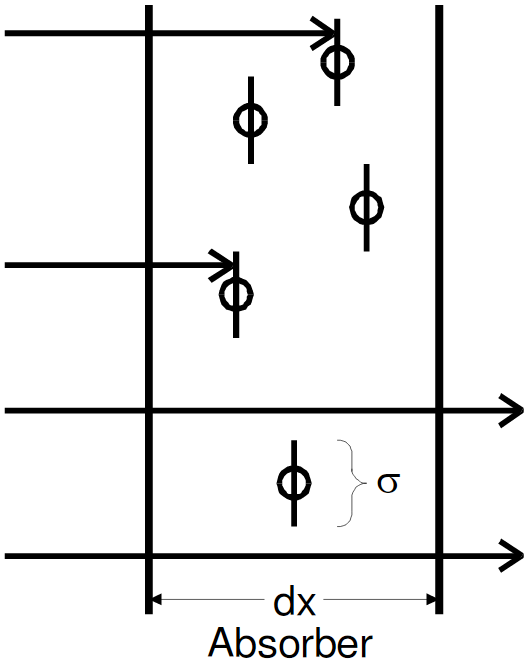
\includegraphics[width=0.3\textwidth]{Bilder/WkeitWW.png}
	\caption{Definition des Wirkungsquerschnitts: Die Pfeile kennzeichnen die Projektile welche auf das Target treffen \cite{V18}.}
	\label{fig:WkeitWW}
\end{figure}



\subsubsection{Der Photoeffekt}
Ein Photon kann ein Elektron aus der Atomhülle schlagen, dafür muss das Photon mindestens die Bindungsenergie $E_\text{B}$ des Elektrons besitzten. Bei diesem Vorgang wird die gesamte Energie $h\nu$ des Photons auf das Elektron übertragen. Das Elektron besitzt also eine kinetische Energie von
\begin{align}
	E_\text{kin} = h\nu - E_\text{B} \ .
\end{align}
Aus Energie-Impuls-Erhaltungsgründen kann dieser Prozess nur in der nähe eines Atomkerns stattfinden. Deshalb werden bevorzugt Elektronen aus der K-Schale ausgelöst (vgl. \cite[3]{V18}). Da sich das Atom nach dem Effekt in einem instabilen Zustand befindet, fallen Elektronen aus höheren Schalen in das enstandene "Loch". Dabei wird Röntgenstrahlung frei welche aber fast komplet in dem Absorber verbleibt. Deshalb kann gesagt werden, dass der Absorber die gesamte Energie des Photons absorbiert. \\
Der Wirkungsquerschnitt $\sigma_\text{Ph}$ des Photoeffekts kann zu
\begin{equation}
	\sigma_\text{Ph} \approx z^{\alpha}\,E^{\delta}
\end{equation}
bestimmt werden. Für den Energiebereich der bei natürlichen Strahlern vorkommt (E < 5\,MeV) ist $4 < \alpha < 5$ und $\delta = -3.5$\ .



\subsubsection{Der Compton- und der Thomson-Effekt}
Der Compton-Effekt ist die inelastische Streuung von Photonen an Elektronen. Das Photon gibt bei dem Stoß mit einem (schwachgebundenen) Elektron aus der Atomhülle einen Teil seiner Energie ab und wird aus der ursprünglichen Bahn herausgelenkt. Die Energie des gestreuten Photons kann Mithilfe des Energie-Impuls-Erhaltungssatzes zu
\begin{align}
	E_{\gamma'} = \frac{E_{\gamma}}{1 + \varepsilon\,(1-\cos(\psi_{\gamma})}
	\label{eqn:Egamma}
\end{align}
bestimmt werden. Dabei ist $E_{\gamma}$ die Energie des Photons vor dem Stoß und $E_{\gamma'}$ ist die Energie nach dem Stoß. $\varepsilon$ entspricht einer normierten Energie $\varepsilon = \frac{E_{\gamma}}{m_0\,c^2}$ und $\psi_{\gamma}$ ist der Streuwinkel des $\gamma$-Quants. Aus Formel \eqref{eqn:Egamma} folgt die Energie $E_\text{l}$ des gestoßenen Elektrons zu
\begin{align}
	E_\text{l} = E_{\gamma} - E_{\gamma'} = E_{\gamma} \frac{\varepsilon\,(1-\cos(\psi_{\gamma})}{1 + \varepsilon\,(1-\cos(\psi_{\gamma})} \ .
	\label{eqn:El}
\end{align}
Der Compton-Effekt ist eine unerwünschte Erscheinung, weil nur ein variierender Bruchteil der Energie des $\gamma$-Quants an den Detektor abgegeben wird (vgl. \cite[5]{V18}). Dadurch entsteht ein kontinuirliches Spektrum, welches schwer zu identifizieren ist. Der über alle Streuwinkel integrierte Wirkungsquerschnitt $\sigma_\text{Co}$ wurde von KLEIN und NISHINA hergeleitet und lautet:
\begin{align}
	\sigma_\text{Co} = \frac{3\,\sigma_\text{Th}}{4} \left( \frac{1+\varepsilon}{\varepsilon^2} \left[\frac{2+2\,\varepsilon}{1+2\,\varepsilon} - \frac{\ln(1+2\,\varepsilon)}{\varepsilon} \right] + \frac{\ln(1+2\,\varepsilon)}{2\,\varepsilon} - \frac{1+3\,\varepsilon}{(1+2\,\varepsilon)^2} \right)
\end{align}
Für sehr kleine Energien $(\varepsilon \ll 1)$ kann $\sigma_\text{Co}$ zu
\begin{align}
	\sigma_\text{Co} = \frac{3\,\sigma_\text{Th}}{4} \left(1 - 2\,\varepsilon + \frac{26}{5}\,\varepsilon^2 + \dots \right)
\end{align}
genähert werden. Für $\varepsilon \rightarrow 0$ geht der Compton-Wirkungsquerschnitt in den Thomsonschen Streuquerschnitt $\sigma_\text{Th}$ über.
\begin{align}
	\sigma_\text{Th} = \frac{8\,\pi}{3}\,r_\text{e}^2
\end{align}
$r_\text{e}$ wird als klassischer Elektronenradius bezeichnet.



\subsubsection{Die Paarbildung}
Bei der Paarbildung wird ein Photon annihilliert und ein Elektron-Positron-Paar erzeugt. Dieser Prozess kann nur in der nähe von einem Atomkern oder einem Elektron als Stoßpartner auftretten, weil sonst die Impulserhaltung nicht gilt. Mit dem Atomkern als Stoßpartner muss die Photonenergie größer als die doppelte Ruheenergie eines Elektrons sein, also
\begin{align*}
	E_{\gamma} > 2\,m_0\,c^2 \ .
\end{align*}
Damit die Paarbildung mit einem Elektron als Stoßpartner stattfinden kann muss das Photon die vierfache Ruheenergie eines Elektrons haben, also
\begin{align*}
	E_{\gamma} > 4\,m_0\,c^2 \ .
\end{align*}
Die kinetische Energie des entstandenen Elektron-Positron-Paares beträgt:
\begin{align}
	\overline{E_{\text{e}^-}} = \overline{E_{\text{e}^+}} = \frac{1}{2}(E_{\gamma} - m_0\,c^2)
\end{align}
Der Wirkungsquerschnitt der Paarbildung $\sigma_\text{Pa}$ hängt von der Kernladungszahl $z$ und der Abschirmung des Coulomb-Feldes ab. Im folgenden werden zwei Grenzfälle betrachtet. Wenn die Paarbildung in Kernnähe auftritt, also bei verschwindender Abschirmung wird der Wirkungsquerschnitt zu
\begin{align}
	&\sigma_\text{Pa} = \alpha\, r_\text{e}^2\, z^2\, \left(\frac{28}{9}\ln(2\,\varepsilon) - \frac{218}{27} \right) \\
	(\alpha = &\text{Sommerfeldsche Feinstrukturkonstante})
	\label{eqn:PaarVerschwindend}
\end{align}
bestimmt. Die Gleichung \eqref{eqn:PaarVerschwindend} ist in einem Energiebereich von $10 < E_\gamma < 25$ MeV gültig. \\
Wenn die Paarbildung am Rand der Elektronenhülle stattfindet, das Coulomb-Feld also vollständig abgeschirmt wird, ergibt sich folgende Gleichung
\begin{align}
	\sigma_\text{Pa} = \alpha\, r_\text{e}^2\, z^2\, \left(\frac{28}{9}\ln\frac{183}{\sqrt[3]{z}} - \frac{2}{27} \right) \ .
\end{align}
Diese ist aber erst ab 500 MeV gültig. \\
Bei der Paarbildung wird die gesamte Energie des Photons in dem Absorber deponiert. Allerdings kann nicht immer die gesamte Energie von dem Detektor gemessen werden, weil dazu Elektron und Positron in den Detektor fallen müssen. Passiert dies nicht, wird keine Energie gemessen. Auch verlieren Elektron und Positron durch Bremsstrahlung Energie, wodurch das Spektrum nach unten verbreitert wird.



\newpage
\subsection{Wirkungsweise eines Halbleiter-Detektors (Germanium-Detektor)}
Halbleiter-Detektoren werden häufig verwendet um ionisierende Strahlung nachzuweisen und die Energie der Strahlung zu bestimmen. Im folgenden wird der Germanium-Detektor für die $\gamma$-Spektroskopie genauer betrachtet. \\
Der wesentliche Bestandteil des Detektors ist eine Halbleiter-Diode. Das bedeutet es gibt einen p- und einen n-dotierten Bereich. Diese Bereiche grenzen aneinander und können freie Ladungsträger (Elektronen und Löcher) austauschen. Die Elektronen und Löcher rekombinieren in den unterschiedlich dotierten Bereichen. Zurück bleiben in der p-Schicht die ortsfesten Akzeptoren und in der n-Schicht die ortsfesten Donatoren \cite[10]{V18}. Diese erzeugen ein elektrisches Potential $U_\text{D}$, wodurch die Elektronen und Löcher nicht mehr rekombinieren können und es entsteht eine ladungsträgerarme Zone. Wie in Abbildung \eqref{fig:Potential} dargestellt ist, kann die ladungsträgerarme Zone durch eine Sperrspannung $U$ vergrößert werden. Im folgenden wird näher darauf eingegangen wie die Verarmungszone vergrößert werden kann.

\begin{figure}[H]
	\centering
	\begin{subfigure}[b]{0.45\linewidth}
		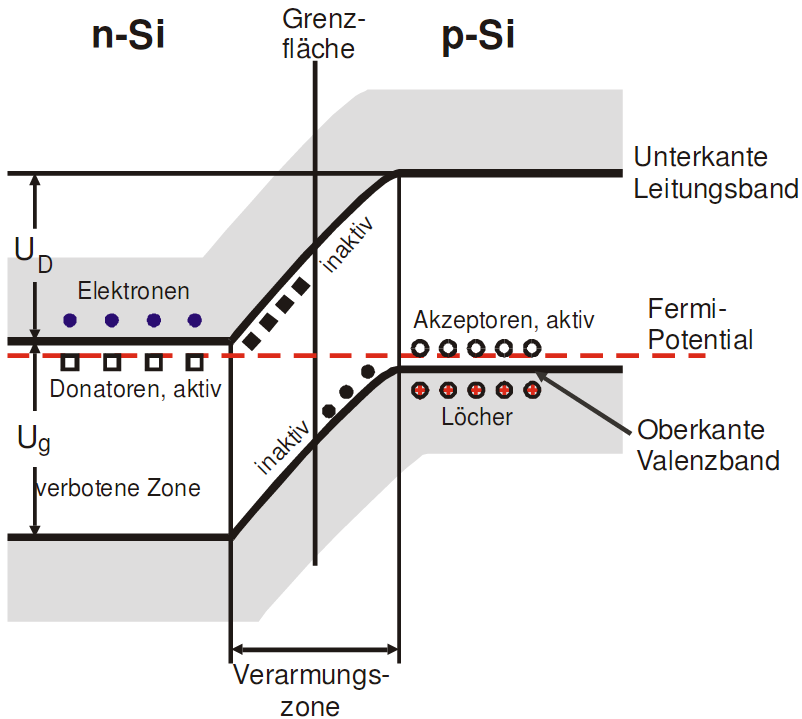
\includegraphics[height=7cm]{Bilder/V1.png}
		\caption{Potentialverhältnis ohne äußere Spannung.}
		\label{fig:Potentiala}
	\end{subfigure}
	\hfill
	\begin{subfigure}[b]{0.45\linewidth}
		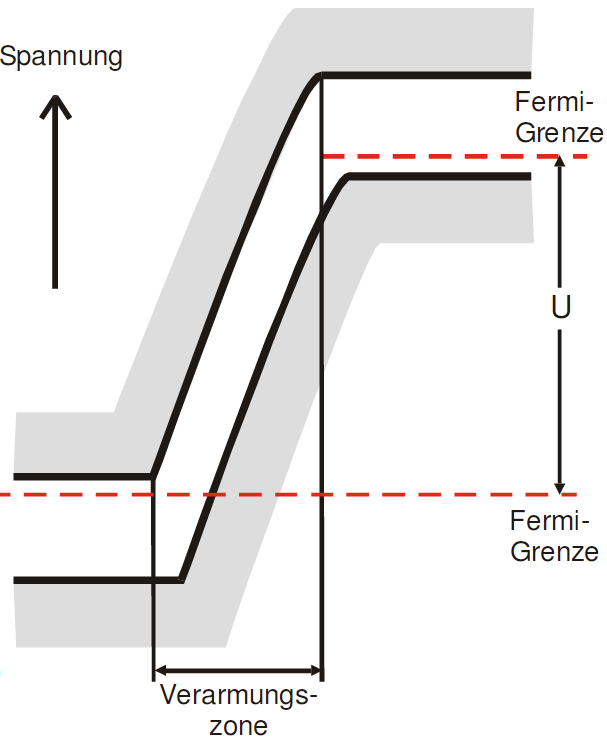
\includegraphics[height=7cm]{Bilder/V2.png}
		\caption{Potentialverhältnis mit äußere Spannung.}
		\label{fig:Potentialb}
	\end{subfigure}
	\caption{Schematische Darstellung der Potentialverhältnisse an einem pn-Übergang \cite{V18}.}
	\label{fig:Potential}
\end{figure}

Wenn ein $\gamma$-Quant in die ladungsträgerarme Zone eindringt kann einer der drei beschriebenen Prozesse eintretten. Das bei diesen Prozessen freigesetzte Elektron stößt auf seinem Weg durch den Festkörper mit vielen anderen Elektronen aus dem Valenzband zusammen. Dabei gibt das freigesetzte Elektron einen Teil seiner Energie zur Erzeugung von Phononen ab. Die restliche Energie wird an die Valenzelektronen abgegeben, wodurch diese in das Leitfähigkeitsband oder darüber hinaus gehoben werden. Es entsteht dadurch ein Elektronen-Loch-Paar, welches durch die anliegende Spannung getrennt wird und einen Ladungsimpuls erzeugen. \\
Die Absorbtionswahrscheinlichkeit (siehe Gl. \eqref{eqn:Absorbtion}) eines $\gamma$-Quants hängt von der Schichtdicke des Absorbermaterials ab. Deshalb ist es besonders wichtig, dass die Verarmungszone so groß wie möglich ist. Dies wird im wesentlichen über eine unsymmetrische Dotierung und die Sperrspannung $U$ gewährleistet. Die Breite der n-Schicht $d_\text{n}$ und die Breite der p-Schicht $d_\text{p}$ sind durch
\begin{align}
	d_\text{n}^2 &= \frac{2\,\varepsilon\,\varepsilon_0} {e_0} \, \frac{U_\text{D} + U}{n_\text{A} + n_\text{D}} \, \frac{n_\text{A}}{n_\text{D}} \\
	d_\text{p}^2 &= \frac{2\,\varepsilon\,\varepsilon_0} {e_0} \, \frac{U_\text{D} + U} {n_\text{A} + n_\text{D}} \, \frac{n_\text{D}}{n_\text{A}}
\end{align}
\hfil {\footnotesize($\varepsilon$ = relative Dielektrizitätszahl, $\varepsilon_0$ = elektrische Feldkonstante)} \hfil \\
gegeben. Um die p-Schicht groß gegenüber der n-Schicht zu machen, wird die Donatordichte $n_\text{D}$ viel größer als die Akzeptordichte $n_\text{A}$ gewählt. Dadurch wird die größe der Verarmungszone zu
\begin{align}
	d = d_\text{p} + d_\text{n} \approx d_\text{p} \approx \sqrt{\frac{2\,\varepsilon\,\varepsilon_0} {e_0} \, \frac{U_\text{D} + U}{n_\text{A}}}
\end{align}
genähert. Es ist also wichtig die Verunreinigung des Absorbers so gering wie möglich zu halten, dies wird über spezielle Kristallzüchtungsverfahren gewährleistet. \\ Außerdem kann die Verarmungszone durch eine möglichst hohe Sperrspannung weiter vergrößert werden. Diese Maßnahme ist allerdings begrenzt, weil in der Verarmungszone Ladungsträger vorhanden sind welche durch thermische Aktivierung entstanden sind. Diese können spontan die Energielücke $E_\text{g}$ (=0.67\,eV bei Ge \cite[13]{V18}) zwischen Valenzband und Leitfähigkeitsband überwinden. Diese Ladungsträger erzeugen einen Leckstrom, welcher als Rauschen gemessen wird. Die Dichte $n_\text{i}$ dieser Ladungsträger ist proportional zu
\begin{align}
	n_\text{i} \propto T^3 \exp\left(-\frac{E_\text{g}}{k_\text{b}\,T} \right) \ .
\end{align}
\hfil {\footnotesize($k_\text{b}$ = Boltzmann Konstante, $T$ = absolute Temperatur)} \hfil \\
Wie aus der Gleichung hervorgeht, kann der Leckstrom durch das herabsetzten der Temperatur des Detektormaterials vermindert werden. \\
Üblicherweise werden Germanium-Detektoren auf $T = 77$\,K abgekühlt. Dadurch kann die Verarmungszone mit einer Sperrspannung von $U = 5$\,kV auf
\begin{align}
	d \approx 3\,\text{cm}
\end{align}
verbeitert werden.



\subsection{Eigenschaften und Kenngrößen eines Halbleiter-Detektors}
Im folgenden werden das energetische Auflösungsvermögen und die Effizienz eines Halbleiter-Detektors bestimmt. Außerdem wird das aufgenommene Spektrum des Detektors beschrieben und daraus die Aktivität der $\gamma$-Quelle bestimmt.



\subsubsection{Energetisches Auflösungsvermögen}
\label{sec:EAuflösung}
Ein Maß für das energetische Auflösungsvermögen ist die Halbwertsbreite $\Delta E_\frac{1}{2}$ der Impulshöhenverteilung. Um zwei Spektrallinien unterscheiden zu können müssen sich deren Mittelwerte mindestens um die Halbwertsbreite unterscheiden. \\
Die Impulshöhenverteilung wird im wesentlichen durch die Anzahl $n$ der Elektron-Loch-Paare festgelegt, die bei der Absorbtion eines $\gamma$-Quants entstehen. Der Mittelwert $\overline{n}$ von $n$ ist gleich dem Quotienten aus der Energie $E_\gamma$ des einfallenden $\gamma$-Quants und der Bildungsenergie $E_\text{El}$ eines Elektron-Loch-Paares \cite[14]{V18}. Die Energielücke $E_\text{g}$ in Germanium beträgt 0.67\,eV, allerdings wird eine Bildungsenergie in Germanium von 2.9\,eV gemessen. Das bedeutet, dass die Bildung von Elektron-Loch-Paaren nur unter der Beteiligung von Phononen möglich ist. Die Energie, die das $\gamma$-Quant an den Detektor abgegeben hat, wird statistisch auf die Phononen- und Elektron-Loch-Paar -Erzeugung verteilt. Dieser Prozess wird durch eine Poisson-Verteilung beschrieben und die Standardabweichung für den unkorrelierten Fall ist durch
\begin{align}
	\sigma = \sqrt{\overline{n}}
\end{align}
gegeben. Allerdings kompensieren sich die Fluktuationen der Ladungsträgererzeugung und der Phononenanregung. Dadurch wird $\sigma$ kleiner, dies wird durch die Einführung des Fano-Faktors $F$ ausgeglichen.
\begin{align}
	\sigma = \sqrt{F\,\overline{n}} = \sqrt{F\,\frac{E_\gamma}{E_\text{El}}}
\end{align}
Für Germanium beträgt $F$ = 0.1 \cite[15]{V18}. Da $n$ sehr viel größer ist als 1, wird die Poisson-Verteilung durch eine Gauß-Verteilung angenähert. Damit folgt für die Halbwertsbreite
\begin{align}
	\Delta E_\frac{1}{2} = \sqrt{8\,\ln2} \, \frac{\sigma} {\overline{n}} E_\gamma = \sqrt{0.8\,\ln2\,E_\gamma \, E_\text{El}} \ .
\end{align}
Das energetische Auflösungsvermögen hängt zusätzlich noch von dem Leckstrom, den Feldinhomogenitäten und dem Verstärkerrauschen (Darauf wird in Kapitel \eqref{sec:} weiter eingegangen) ab. Diese Effekte sind unkorreliert, deshalb kann die Gesamthalbwertsbreite zu
\begin{align}
	H_\text{ges}^2 = \Delta E_\frac{1}{2}^2 + H_\text{R}^2 + H_\text{I}^2 + H_\text{E}^2
\end{align}
zusammengesetzt werden. $H_\text{R}$ ist die Halbwertsbreite des Leckstroms, $H_\text{I}$ ist die Halbwertsbreite der Feldinhomogenität und $H_\text{E}$ ist die Halbwertsbreite des Verstärkerrauschens. Der Leckstrom und das Verstärkerrauschen können durch abkühlen deutlich vermindert werden. Auch muss die Sperrspannung eine Mindesthöhe überschreiten (U > Depletionsspannung).



\subsubsection{\texorpdfstring{$\gamma$}{}-Spektrum eines Germanium-Detektors}
In Abbildung \eqref{fig:Spektrum} ist das Spektrum eines monochromatischen $\gamma$-Strahlers aufgenommen.

\begin{figure} % y-Spektrum
	\centering
	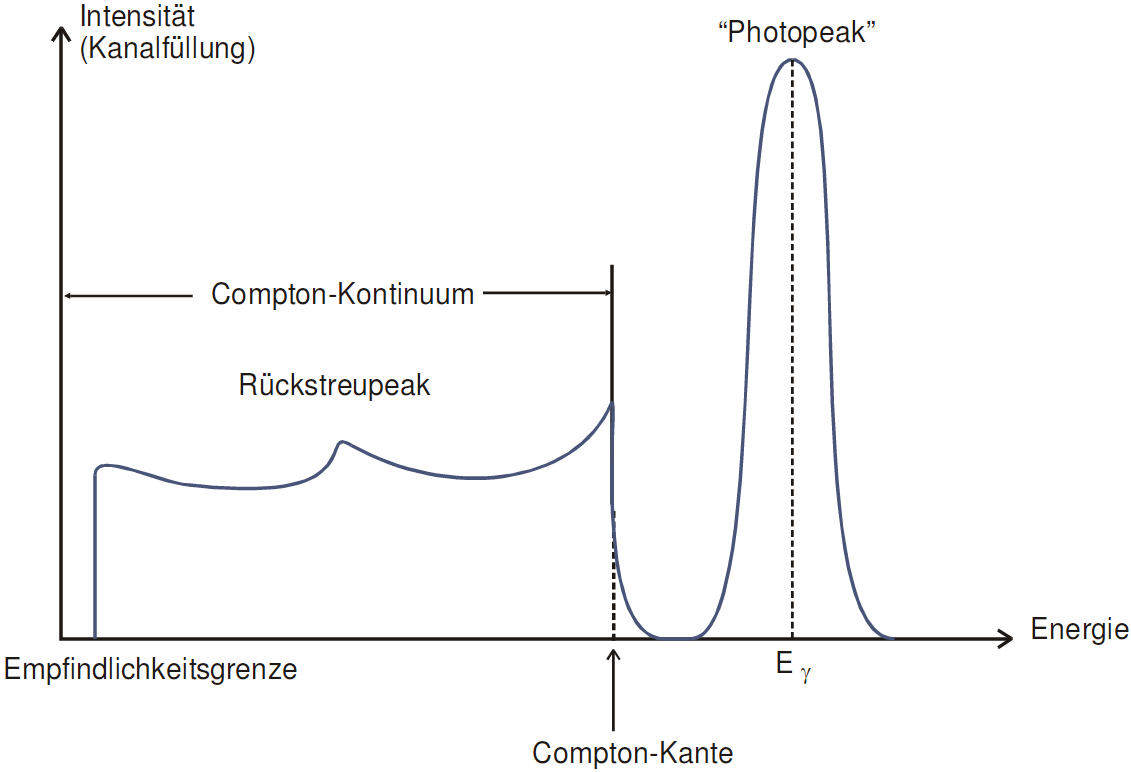
\includegraphics[width=0.8\linewidth]{Bilder/Spektrum.png}
	\caption{Das $\gamma$-Spektrum eines Germanium-Detektors \cite{V18}.}
	\label{fig:Spektrum}
\end{figure}

Das Spektrum besteht aus dem Photopeak, dem Compton-Kontinuum und dem Rückstreupeak. Der Photopeak entsteht wenn der Photoeffekt an der Absorbtion beteiligt ist. Dabei wird die gesamte Energie des $\gamma$-Quants an den Absorber abgegeben. Seine Halbwertsbreite ist, wie in Kap.\ref{sec:EAuflösung} dargelegt, ein Maß für die Energieauflösung des Detektors \cite[22]{V18}. \\
Das Compton-Kontinuum ist ein störender Bereich bei der $\gamma$-Spektroskopie. Dieser Bereich reicht von 0 bis zur Compton-Kante $E_\text{e,max} = E_\gamma \, \frac{2\,\varepsilon} {1 + 2\,\varepsilon}$. Er entsteht durch die Compton-Streuung an den Elektronen. Der Rückstreupeak liegt in dem Compton-Kontinuum und entsteht durch Quanten die nicht direkt in den Detektor fallen. Beispielsweise Quanten die an der Pb-Abschirmung oder der Quelle selbst getreut werden. Der Ort des Rückstreupeaks kann durch einsetzten von 180° in Gleichung \eqref{eqn:Egamma} abgeschätzt werden.



\subsubsection{Aktivitäts- und Energiebestimmung einer \texorpdfstring{$\gamma$}{}-Quelle}
Für die Energiebestimmung eines einzelnen Peaks muss zunächst der Detektor kalibriert. Dazu wird ein $\gamma$-Strahler mit bekannten Energien aufgenommen. Damit wird den Kanälen des Vielkanalanalysators eine Energie zugeordnet. Um die Fehler der linearen Regression zu minimieren wird ein linienreiches Spektrum benötigt. \\
Zur Bestimmung der Aktivität $A$ muss zunächst die Effizienz $Q$ durch eine Kalibrierungsmessung ermittelt werden. Die Effizienz ist die Nachweißwahrscheinlichkeit eines Quants mit einer Energie $E_\gamma$. Dafür wird ein $\gamma$-Strahler mit bekannter Aktivität verwendet und mit dem gemessenen Zählergebnis $Z$ in Verbindung gebracht.
\begin{align}
	Z = \Omega\,A\,W\,Q
\end{align}
Da die Strahlung Kugelförmig aus dem Strahler austritt, wird nur ein kleiner Teil der Strahlung in dem Detektor aufgenommen. Diese Größe wird durch den Raumwinkel $\Omega$ beschrieben. $W$ ist die Emissionswahrscheinlichkeit einer bestimmten Energie bei Mehrlinienstrahlern. Um die Effizienz zu bestimmen müssen also $A$, $Z$, $W$ und $\Omega$ bekannt sein. Die Aktivität wird aus Herstellerangaben entnommen und das Zählergebnis aus einer Messung. Die Emissionswahrscheinlichkeit kann einschlägigen Tabellen entnommen werden \cite{V18}. Der Raumwinkel kann über
\begin{align}
	\Omega = 2\,\pi\,\left(1 - \frac{a}{\sqrt{a^2 + r^2}} \right)
\end{align}
\hfil {\footnotesize($a$ = Abstand zwischen Quelle und Detektor, $r$ = Detektorradius)} \hfil \\
berechnet werden. Solbald die Effizienz bestimmt wurde kann die Energie und die Aktivität von unbekannten Strahlern bestimmt werden.









\subsection{Fehlerrechnung}
Sämtliche Fehlerrechnungen werden mit Hilfe von Python 3.4.3 durchgeführt.
\subsubsection{Mittelwert}
Der Mittelwert einer Messreihe $x_\text{1}, ... ,x_\text{n}$ lässt sich durch die Formel
\begin{equation}
	\overline{x} = \frac{1}{N} \sum_{\text{k}=1}^\text{N} x_k
	\label{eqn:ave}
\end{equation}
berechnen. Die Standardabweichung des Mittelwertes beträgt
\begin{equation}
	\Delta \overline{x} = \sqrt{ \frac{1}{N(N-1)} \sum_{\text{k}=1}^\text{N} (x_\text{k} - \overline{x})^2}
	\label{eqn:std}
\end{equation}

\subsubsection{Gauß'sche Fehlerfortpflanzung}
Wenn $x_\text{1}, ..., x_\text{n}$ fehlerbehaftete Messgrößen im weiteren Verlauf benutzt werden, wird der neue Fehler $\Delta f$ mit Hilfe der Gaußschen Fehlerfortpflanzung angegeben.
\begin{equation}
	\Delta f = \sqrt{\sum_{\text{k}=1}^\text{N} \left( \frac{ \partial f}{\partial x_\text{k}} \right) ^2 \cdot (\Delta x_\text{k})^2}
	\label{eqn:var}
\end{equation}

\subsubsection{Lineare Regression}
Die Steigung und y-Achsenabschnitt einer Ausgleichsgeraden werden gegebenfalls mittels Linearen Regression berechnet.
\begin{equation}
	y = m \cdot x + b
	\label{eqn:reg}
\end{equation}
\begin{equation}
	m = \frac{ \overline{xy} - \overline{x} \overline{y} } {\overline{x^2} - \overline{x}^2}
	\label{eqn:reg_m}
\end{equation}
\begin{equation}
	b = \frac{ \overline{x^2}\overline{y} - \overline{x} \, \overline{xy}} { \overline{x^2} - \overline{x}^2}
	\label{eqn:reg_b}
\end{equation}
